\chapter{Incorporating Spatial Effects}
\label{chap4}

\hspace{\parindent} After analysing the model, it was then compared to real applause.
The applause duration of varying audience sizes were taken from Youtube videos of musical concerts and performances.
The applause duration was manually recorded.
The audience size was either taken from the seating capacity and/or ticket sales for the given concert/performance, or was estimated by the area or room the audience resided in.
The relationship of the data set was tested with both applause duration and population size in order to find an appropriate linear dependence, as shown in figure \ref{fig:realclap}.

\begin{figure}[h]
  \centering
  \begin{subfigure}[b]{0.4\linewidth}
    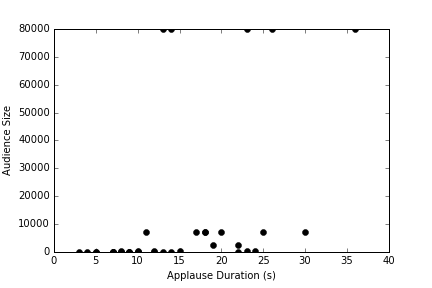
\includegraphics[width=\linewidth]{images/chapter4/1.png}
    \caption{Graphing size versus applause duration.}
  \end{subfigure}
  \begin{subfigure}[b]{0.4\linewidth}
    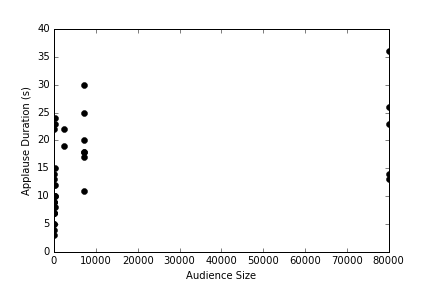
\includegraphics[width=\linewidth]{images/chapter4/2.png}
    \caption{Graphing applause duration versus size.}
  \end{subfigure}
    \begin{subfigure}[b]{0.4\linewidth}
    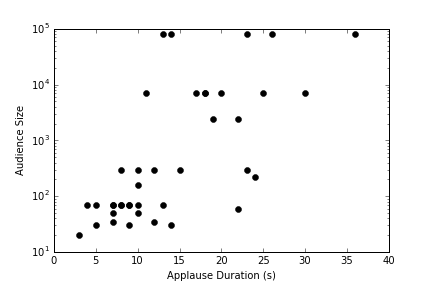
\includegraphics[width=\linewidth]{images/chapter4/3.png}
    %\label{fig:nonTrivSim}
    \caption{Graphing size (in the logarithmic scale) versus applause duration}
  \end{subfigure}
    \begin{subfigure}[b]{0.4\linewidth}
    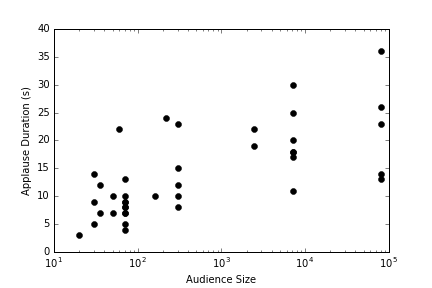
\includegraphics[width=\linewidth]{images/chapter4/4.png}
    %\label{fig:nonTrivSim}
    \caption{Graphing applause duration versus size (in the logarithmic scale).}
  \end{subfigure}
  \caption{Different graphs of the data points of real-life applause.}
  \label{fig:realclap}
\end{figure}

Figure \ref{fig:realclap} (d) makes the most sense; the applause duration of the audience is dependent on the size of the audience.
The question now is whether or not the compartmental model can recreate \ref{fig:realclap} (d).
The current model shows no population size dependence; changing the population size does not affect the applause duration for a given set of parameters.
This is because of the assumption that the network is fully connected, meaning that an audience member in front is influenced the exact same way by the whole audience as an audience member at the back.
As this does not seem to be the case in real-life applause, spatial effects must be incorporated by modifying the feedback function $f'(\alpha)$.

\section{Different configurations for field of vision}

\hspace{\parindent}The field of view configurations represent the audience members that may influence the reference agent.
In real life, the  reference agent is influenced by a limited number of audience members, not the whole audience.
The network is no longer fully-connected, observing a modified, extended Moore neighborhood.
It is extended since it considers all agents till the front row of the system, and not just those $1$ unit away.
It is modified since it does not consider all directions; the directions considered are affected by the configuration.
$\theta = 0$ represents all audience members only directly in front of the reference agent until the very front. 
$\theta = \pi$ represents all rows ahead of the reference agent. 
$\theta = \frac{\pi}{2}$ considers all agents from the north-east direction to the north-west in a $90$ degree arc. The configurations are shown in figure \ref{fig:spaceconfig}.

\begin{figure}[h]
  \centering
  \begin{subfigure}[b]{0.3\linewidth}
    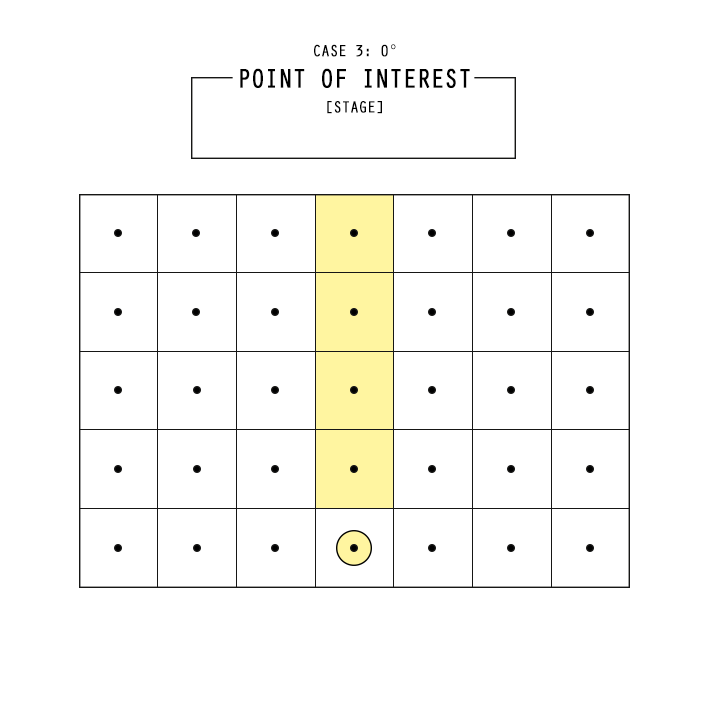
\includegraphics[width=\linewidth]{images/chapter4/0degD.png}
    \caption{$\theta = 0$}
  \end{subfigure}
  \begin{subfigure}[b]{0.3\linewidth}
    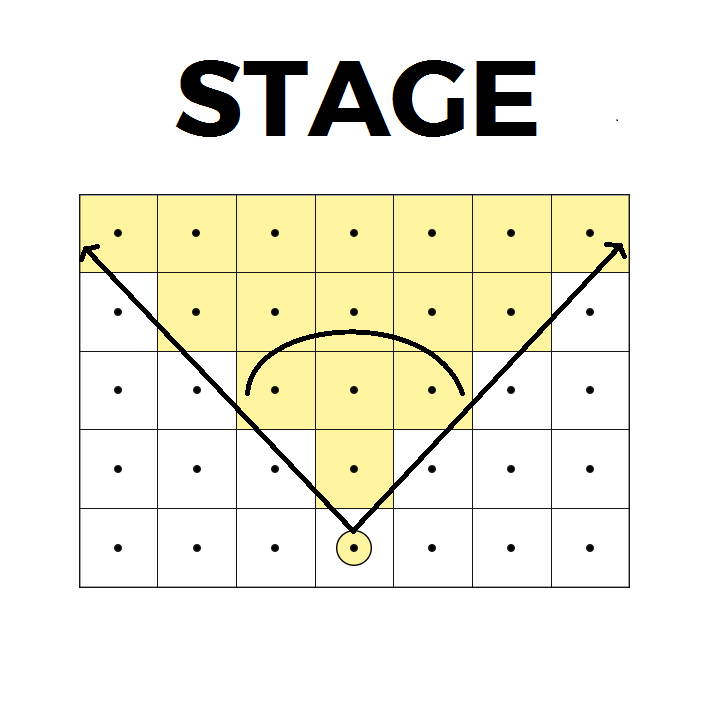
\includegraphics[width=\linewidth]{images/chapter4/90degD.png}
    \caption{$\theta = \frac{\pi}{2}$}
  \end{subfigure}
    \begin{subfigure}[b]{0.3\linewidth}
    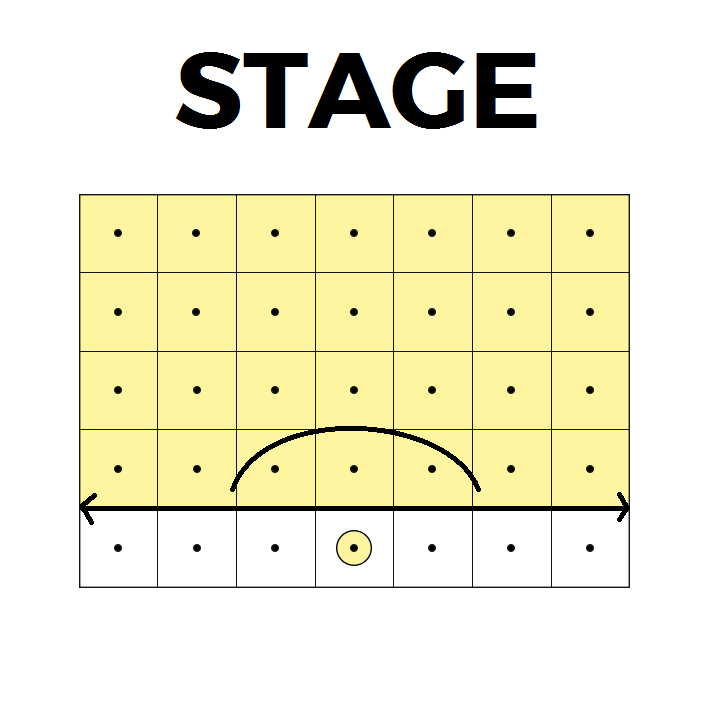
\includegraphics[width=\linewidth]{images/chapter4/180degD.png}
    %\label{fig:nonTrivSim}
    \caption{$\theta = \pi$}
  \end{subfigure}
  \caption{Different field-of-view configurations. The encircled black dot shaded in yellow is the reference agent. The boxes highlighted in yellow are what can influence the  encircled reference agent.}
  \label{fig:spaceconfig}
\end{figure}

\section{Simulating the different spatial configurations}

\hspace{\parindent} Initially, $f'(\alpha)$ bases the fraction of $n_{c}$ throughout the whole population. After incorporating spatial effects, that fraction is only within the field-of-view of the reference agent.
The feedback function is still parametrized by $\alpha$.
%The code developed is provided in Appendix \ref{apndx:spacesim}.

\begin{figure}[h]
  \centering
  \begin{subfigure}[b]{0.4\linewidth}
    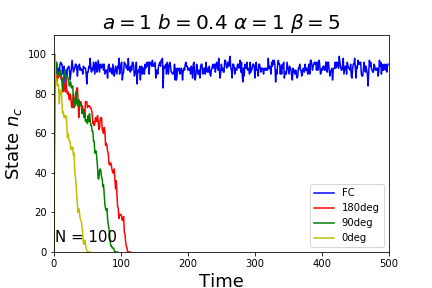
\includegraphics[width=\linewidth]{images/chapter4/feedback_sim4.png}
    \caption{Comparing simulations with spatial effects to the original fully-connected simulation.}
  \end{subfigure}
  \begin{subfigure}[b]{0.4\linewidth}
    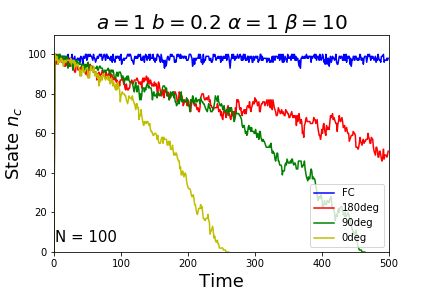
\includegraphics[width=\linewidth]{images/chapter4/feedback_sim5.png}
    \caption{$\theta = 180$ has yet to reach steady-state but is steadily heading towards $0$.}
  \end{subfigure}
    \begin{subfigure}[b]{0.4\linewidth}
    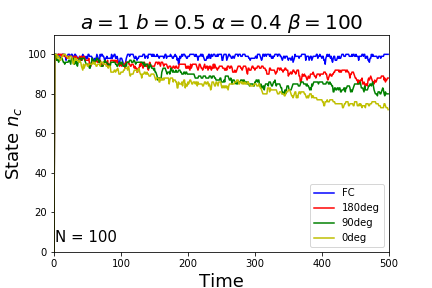
\includegraphics[width=\linewidth]{images/chapter4/feedback_sim6.png}
    %\label{fig:nonTrivSim}
    \caption{All simulations are slowly reaching steady-state.}
  \end{subfigure}
    \begin{subfigure}[b]{0.4\linewidth}
    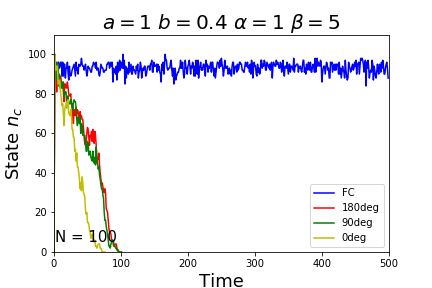
\includegraphics[width=\linewidth]{images/chapter4/feedback_sim3.png}
    %\label{fig:nonTrivSim}
    \caption{A case where $\theta = \frac{\pi}{2}$ is similar to $\theta = 0$.}
  \end{subfigure}
    \begin{subfigure}[b]{0.4\linewidth}
    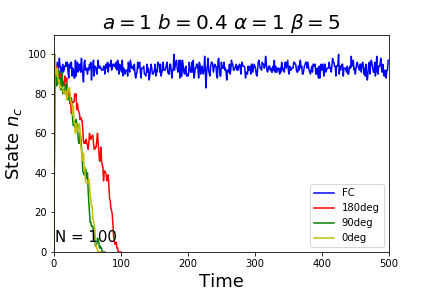
\includegraphics[width=\linewidth]{images/chapter4/feedback_sim2.png}
    %\label{fig:nonTrivSim}
    \caption{A case where $\theta = \frac{\pi}{2}$ is similar to $\theta = \pi$.}
  \end{subfigure}
  \begin{subfigure}[b]{0.4\linewidth}
    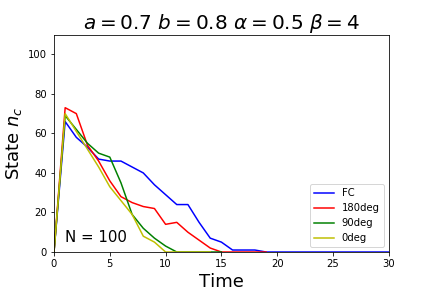
\includegraphics[width=\linewidth]{images/chapter4/feedback_sim7.png}
    %\label{fig:nonTrivSim}
    \caption{All configurations have a trivial steady-state $0$.}
  \end{subfigure}
  \caption{Different graphs comparing effect of different feedback functions under different parameters.}
  \label{fig:spacesim}
\end{figure}

Shown in figure \ref{fig:spacesim} are simulations with different parameters ($a,b,\alpha,\beta$) comparing the different feedback functions, the original fully-connected network, $\theta = \pi$, $\theta = \frac{\pi}{2}$, and $\theta = 0$.
Graphs (a), (b), and (c) show that in our system, feedback functions are less effective in less connected networks. 
There is clearly a downward trend when it comes to applause duration.
Graphs (d) and (e) show that $\theta = \frac{\pi}{2}$ can be similar to either remaining configurations, as well as be somewhere in between.
Generally, simulations incorporating any form of field-of-view feedback do not have a non-trivial steady-state.
Graphs (b) and (c) show cases where the simulations have not ended, but exhibit an obvious downward trend.
Given more iterations, the simulations would end, unlike the fully-connected ones.
Graph (g) shows a special case where all simulations have a trivial steady-state of zero.
One thing to note is that the analysis done for the fully-connected system (phase space graphs, critical and unstable points) cannot be applied to the systems with spatial effects.
A different steady-state equation must be setup to reflect how each agent is influenced differently.
Such analysis will no longer be pursued as it is outside the scope of the study.

\section{Finding the parameters $(a,b,\alpha,\beta)$ for real-life applause}

\hspace{\parindent}Recalling, incorporating spatial effects to the feedback function effectively reduces the number of agents influencing a reference agent. Increasing the population size should increase the feedback since the agents in the back row of a 100x100 grid should 'see' more people than those in the back row of a 10x10 grid. 
This effectively eliminates the original problem of the fully-connected network being scale free.
It is now possible for the applause duration to be dependent on the population.
This phenomena is investigated by simulating a set of parameters $(a,b,\alpha,\beta)$ with varying populations.
For simplicity, the system grid will always be a 2-dimensional lattice of equal lengths.
Also, the spatial configuration used will be $\theta = \pi$.
The total population sample will be perfect squares ranging from $10^1$ to $10^4$.

%The code developed is provided in Appendix \ref{apndx:popdep}.

For this case, each iteration is considered  $1$ second.
Five trials were performed per sample population.
Due to insufferable run times, if a parameter set $(a,b,\alpha,\beta,N)$ returned a trial with applause duration greater than $60$ seconds, it is marked as $0$ seconds and no further trials are performed.
This means that graphs with data points of $0$ seconds are to be disregarded.

\begin{figure}[h]
  \centering
  \begin{subfigure}[b]{\linewidth}
    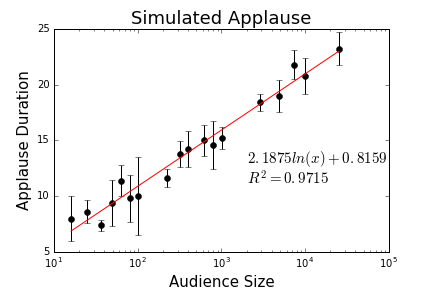
\includegraphics[width=\linewidth]{images/chapter4/sim.png}
    \caption{Simulated points showing population size dependence.}
  \end{subfigure}
  \begin{subfigure}[b]{\linewidth}
    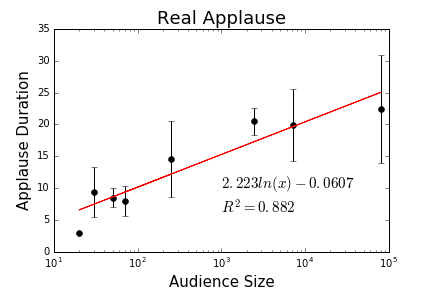
\includegraphics[width=\linewidth]{images/chapter4/real.png}
    \caption{Real-life data points on population size dependence.}
  \end{subfigure}
  \caption{Comparing the simulated and actual graph of applause duration versus population size. Both increase linearly in the logarithmic scale.}
  \label{fig:durXsizComp}
\end{figure}

Shown in figure \ref{fig:durXsizComp} is the parameter set $(a=1,b-0.7,\alpha=0.8,\beta=1)$ that best recreates the real-life applause. 
This was found by simply generating the applause duration versus audience size graph for every parameter set, then comparing its fitting function with that of the real applause. 
Similar parameter sets are shown in the appendix (\ref{apndx:bestfit})
Though this is the best fit parameter set, it still does not fully emulate the real applause.
As seen, the data points for the real-life applause is more deviant compared to the simulation.
The model may still be incomplete, or the data points for real-life applause is not enough.
On reason for this is that the data points for real applause is not enough.
Data acquisition was difficult due to a duration-size uncertainty.
For big audience sizes, the size is well defined because of the seating capacity of the stadium or the ticket sales for the event. 
Applause duration is very uncertain because it is very hard to determine when the applause starts and ends due to the sheer amount of people.
Also, at no point does the crowd go completely silent, making it hard to distinguish applause from cheers and screems.
For small audience sizes, the applause is well defined since it is clearly audible in the video, and can also be visually confirmed.
The audience size is uncertain because the videos of small audience sizes are either street performances or room performances.
For street perfomances, people come and go.
For room performances, the videographer is focused on the performer, thus the audience size cannot be confirmed with absolute certainty and must be estimated.
Another source for error is the spatial configuration. 
The given setup only accounts for sight. A box with the reference agent at the center can be added in order to account for audible influence.
Finally, the assumption that everyone claps after the performance does not encapsulate all forms of audience applause.
This aspect can included by varying the forcing function to different probabilities, instead of 100%.
An in-depth analysis on the new model is also warranted.

